\documentclass[final,twoside,11pt,titlepage,a4paper,english,bibliography=totocnumbered,listof=numbered]{scrbook}

\usepackage{tikz}
\usepackage{pgfgantt}

\def\pic{
  \clip (0,0) rectangle (2,2);
  \definecolor{LightBlue}{rgb}{0.55,0.55,1}
  \definecolor{DarkBlue}{rgb}{0.2,0.2,0.5}
  \filldraw[fill=gray!20,draw=white] (0,0) [very thick]rectangle (1,1);
  \filldraw[fill=gray!20,draw=white] (1,1) [very thick]rectangle (2,2);
  \filldraw[fill=LightBlue,draw=white] (0,1) [very thick]rectangle (1,2);
}

\usepackage{color}
\definecolor{LightBlue}{rgb}{0.55,0.55,1}
\definecolor{DarkBlue}{rgb}{0.2,0.2,0.5}

\newenvironment{itemize3}{
\begin{itemize}
  \setlength{\itemsep}{1pt}
  \setlength{\parskip}{0pt}
  \setlength{\parsep}{0pt}
}{\end{itemize}}

\newenvironment{itemize2}{
\begin{itemize}
  \setlength{\itemsep}{1pt}Aussagekraft
  \setlength{\parskip}{0pt}
  \setlength{\parsep}{0pt}
}{\end{itemize}}

\newenvironment{description2}{
\begin{description}
  \setlength{\itemsep}{1pt}
  \setlength{\parskip}{0pt}
  \setlength{\parsep}{0pt}
}{\end{description}}

\newenvironment{enumerate2}{
\begin{enumerate}
  \setlength{\itemsep}{1pt}
  \setlength{\parskip}{0pt}
  \setlength{\parsep}{0pt}
}{\end{enumerate}}

\newcommand{\STYLEfootnotetext}{\begin{minipage}{.4\textwidth}\scriptsize Learning Technologies\\LuFG Informatik 9\\RWTH Aachen University\end{minipage}}

\newcommand{\STYLEleftpicture}{
  \vspace{-11.6mm}
  \begin{tikzpicture}[xscale=-1,scale=.75]
    \pic
  \end{tikzpicture}}
\newcommand{\STYLErightpicture}{
  \vspace{-11.6mm}
  \begin{tikzpicture}[scale=.75]
    \pic    
  \end{tikzpicture}
}

\newcommand{\tit}{Native Visualization of Mobile Activity Patterns}
\newcommand{\keywords}{KEYWORDS}
\newcommand{\keymore}{}
\newcommand{\auth}{Christian Jan\ss en}
\newcommand{\type}{Bachelor Thesis}


% Leichte Variation von http://hci.rwth-aachen.de/karrer_thesistemplate
% Weiter leichte veränderungen für Mo - v=0.9b
% =============
% = Changelog =
% =============
% [0.99b]
% new - DotVarDescription environment: Adds dots between label and description.
% new - Addes some listings styles from Max Speicher (@maxspeicher) for the listings package and some additional from Gregor Aisch.
% changed - VarDescription: The description label is not aligned to the left.
%
% [0.98b]
% changed - styling of headings (section to subparagraph) from titleformat to addtokomafont so it is
%           possible to change the style with \addtokomafont{\Large} etc. from the main document.
%
% [0.97b]
% new - abstract environment -> \begin{abstract}[name (default none)] TEXT \end{abtract}
% new - acknowledgments environment -> \begin{acknowledgments}[Acknowledgments] TEXT \end{acknowledgments}
%
% [0.96b]
% new - compatibility with scrbook \part command (sectsty package is incompatible)
% removed - sectsty package (replaced functionality with titlesec commands)
%
% [0.953b]
% new - added hyphen option to url-package to allow line breaks after hyphens "-" in urls
%
% [0.952b]
% changed - automatically set header to 'Bibliography' with \printbibliography
%
% [0.951b]
% new - bibliography heading changable with \def\bibheadingonline{TEXT} and \def\bibheadingoffline{TEXT}
% changed - \mnote color (light blue) and \mnote fontsize normal changeable to footnotesize with \def\mnotefootnotesize{}
% changed - Seperate bibliography titles - references -> References
%
% [0.95b]
% new - changed to biblatex
% new - command \setwidesite to be called before \printbibliography to increase side width
% new - biblatex filter online (@online) and offline (!@online)
% dep - \widebibliography
%
% [0.9b]
% new - \usepackage{soul} for higlighting (\hl{some text} etc.)
% new - \shl{some text} to mark text red, no background marking
%
% [0.85b]
% new - Environment VarDiscription | \begin{VarDescription}{widest word}
% new - \widebibliography{} command
% new - scenario list (alph label and only 2pt item seperation)
% changed - changed seperator between multiple citations from ',' to ';'
% changed - changed labels in itemize list
% changed - csquote style to american (starts quotations with double quote instead of single quotes (inverted commas)).
% changed - csquote cite command to use natbibs \citep command.
%
% [0.8b]
% new - \footcite[]{} command
% new - Changed color of item/enum and description label to LightBlue



\usepackage[hyphens]{url}

%
%   B I B L I O G R A P H Y   &   C I T A T I O N S
%
%\usepackage[square]{natbib}  % round?
% \usepackage[round]{dinat}

% \usepackage{bibgerm}
% \usepackage{natbib}
% \bibliographystyle{plainnat}
% \bibliographystyle{gerapali}
% \bibliographystyle{natdin}
% \bibliographystyle{natdineng}
% \bibpunct{(}{)}{;}{a}{,}{,}
% \bibpunct{[}{]}{,}{a}{,}{,}
% \bibpunct{[}{]}{;}{a}{,}{,}
% \newcommand{\fullcite}{\cite}
% \newcommand{\footcite}[2][]{\footnote{#1 \citet{#2}}}

% ============
% = BibLaTeX =
% ============
% natbib for compability with natbib style citing and authoryear type
\usepackage[style=numeric,natbib=true]{biblatex}
% \usepackage[style=alphabetic,natbib=true]{biblatex}
% \usepackage[style=authoryear,natbib=true]{biblatex}
% \usepackage[style=authoryear,natbib=true, useprefix=true]{biblatex}

\renewcommand{\bibsetup}{%
  \markboth{\MakeUppercase{Bibliography}}{}
}

\newcommand{\setwidesite}{%
  \fancyhfoffset[LE,RO]{\marginparsep+\marginparwidth-4cm}
  \fancyheadoffset[LO,RE]{0cm}
  \fancyfootoffset[RE]{2cm}
  \newgeometry{inner=2cm, outer=2cm, bottom=4cm}}

\ifdefined\bibheadingonline
  \defbibheading{online}{\section*{\bibheadingonline}}
\else
  \defbibheading{online}{\section*{Online References}}
\fi
\ifdefined\bibheadingoffline
  \defbibheading{offline}{\section*{\bibheadingoffline}}
\else
  \defbibheading{offline}{\section*{Printed References}}
\fi

\defbibfilter{online}{%
  \( \type{online} \)}

\defbibfilter{offline}{%
  \( \not \type{online} \)}
  
% \DeclareNameFormat{sortname}{%
%   \iffirstinits
%   {\usebibmacro{name:last-first}{#1}{#4}{#5}{#7}}
%   {\usebibmacro{name:last-first}{#1}{#3}{#5}{#7}}%
%   \usebibmacro{name:andothers}}
  




%
% LANGUAGE & ENCODING
%
\usepackage[english]{babel}
% \usepackage[ngerman]{babel}
% Bug: this statement seems to be useless, instead, the _last_
% language from the parameterlist to \usepackage{babel} seems to be
% important
% \selectlanguage{ngerman}
\selectlanguage{english}
\usepackage[T1]{fontenc}
% \usepackage[latin1]{inputenc}   % can use native umlauts
\usepackage[utf8]{inputenc}   % can use native umlauts
% \usepackage[babel,german=quotes]{csquotes}  % provides \enquote{Blupp} => "`Blupp"'
\usepackage[babel,english=american]{csquotes}	% provides \enquote{Blupp} => "`Blupp"'
% \SetCiteCommand{\citep}
\SetCiteCommand{\parencite} % Changed for biblatex

\usepackage{units}              % unified way of setting values with units

\usepackage{appendix}
% \renewcommand{\appendixpagename}{Anhänge}
% \renewcommand{\appendixtocname}{Anh"ange}
%
% FONTS
%
% \usepackage{times}              % use times font
% \usepackage{lmodern}            % use lmodern fonts
%change standard fonts to Palatino and Helvetica
% \usepackage{palatino}
\usepackage{mathpazo} 
\usepackage[scaled=.95]{helvet} 
\usepackage{courier} 

\usepackage{noindent} %do not indent at new paragraphs but add a vertical offset

\usepackage{url}

%
% SYMBOLS
%
% \usepackage[right]{eurosym}
\usepackage{gensymb}
\usepackage{textcomp}           % for \textmu (non-italic $\mu$)
% \usepackage{marvosym}
\makeatletter					% make "@" a regular letter, not a special symbol


%\setcounter{secnumdepth}{3}     % limit enumeration depth
%\setcounter{tocdepth}{3}        % limit TOC depth

% tables & table formatting
\usepackage{tabularx}
\usepackage{booktabs}
\usepackage{multirow}
% \usepackage{dcolumn}%D{,}{,}{Nachkommastellen}

% \setlength{\itemsep}{5mm plus10mm minus20mm}


\fboxsep0mm

\usepackage{amsmath}            % math fonts
\usepackage{amssymb}            % math symbols
\usepackage{setspace}           % line spacing 

% package for higlighting etc. (\hl{}...)
\usepackage{soul}

% simple highlight without soul package
\newcommand{\shl}[1]{\textcolor{red}{#1}}

%
% C O D E   L I S T I N G S
%

%\usepackage{fancyvrb}           % algorithm-boxes
\usepackage{listings}

% \lstset{
%   numbers=left,
%   numberstyle=\tiny,
%   numbersep=5pt,
%   breaklines=true,
%   stepnumber=5,
%   tabsize=2,
%   basicstyle=\ttfamily\small,
%   frame=none,
%   numberfirstline=true,
%   firstnumber=1
%   }
% ============================
% = Listings Styles from Max =
% ============================

\definecolor{violet}{cmyk}{0.45,0.97,0.27,0.21}
\definecolor{lstblue}{cmyk}{1,0.80,0,0}
\definecolor{lstgreen}{cmyk}{0.71,0.21,0.65,0.22}
\definecolor{bluegrey}{cmyk}{0.56,0.24,0.11,0.05}
\definecolor{javadoc}{cmyk}{0.88,0.59,0,0}
\definecolor{lstgrey}{cmyk}{0.55,0.44,0.42,0.32}

\lstdefinelanguage{SQL}{
     keywords={},
     keywordstyle=\color{bluegrey}\bfseries,
     morekeywords=[2]{CREATE,TABLE,IF,NOT,EXISTS,NULL,SET,DEFAULT,PRIMARY,KEY,COLLATE,CHARACTER,AUTO_INCREMENT,ENGINE,CHARSET},
     keywordstyle={[2]\color{violet}\bfseries},
     otherkeywords={int,varchar,double,text,tinyint},
     sensitive=false,
     morecomment=[l][\color{lstgreen}]{//},
     morecomment=[s][\color{lstgreen}]{/*}{*/},
     morecomment=[s][\color{javadoc}]{/**}{*/},
     morestring=[b]',
     morestring=[b]"
  }
\lstdefinelanguage{PHP}{
     keywords={},
     keywordstyle=\color{bluegrey}\bfseries,
     morekeywords=[2]{static,function,if,return,pow,sin,cos,asin,min,sqrt,int},
     keywordstyle={[2]\color{violet}\bfseries},
     otherkeywords={@param, @returns, @author, @type, @link, @see},
     sensitive=false,
     morecomment=[l][\color{lstgreen}]{//},
     morecomment=[s][\color{lstgreen}]{/*}{*/},
     morecomment=[s][\color{javadoc}]{/**}{*/},
     morestring=[b]',
     morestring=[b]"
  }
\lstdefinelanguage{JavaScript}{
     keywords={},
     keywordstyle=\color{bluegrey}\bfseries,
     morekeywords=[2]{attributes, class, classend, do, empty, endif, endwhile, fail, function, functionend, if, implements, in, inherit, inout, not, of, operations, out, return, set, then, types, while, use},
     keywordstyle={[2]\color{violet}\bfseries},
     otherkeywords={@param, @returns, @author, @type, @link, @see},
     sensitive=false,
     morecomment=[l][\color{lstgreen}]{//},
     morecomment=[s][\color{lstgreen}]{/*}{*/},
     morecomment=[s][\color{javadoc}]{/**}{*/},
     morestring=[b]',
     morestring=[b]"
  }
\lstdefinelanguage{Java}{
     keywords={},
     keywordstyle=\color{bluegrey}\bfseries,
     morekeywords=[2]{abstract,boolean,break,byte,case,catch,char,class,
      const,continue,default,do,double,else,extends,false,final,
      finally,float,for,goto,if,implements,import,instanceof,int,
      interface,label,long,native,new,null,package,private,protected,
      public,return,short,static,super,switch,synchronized,this,throw,
      throws,transient,true,try,void,volatile,while},
     keywordstyle={[2]\color{violet}\bfseries},
     morekeywords=[3]{@SuppressWarnings, @Capability, @Override},
     keywordstyle={[3]\color{lstgrey}},
     otherkeywords={@param, @return, @returns, @author, @link, @see},
     sensitive,
     morecomment=[l]//,
     morecomment=[s]{/*}{*/},
     morecomment=[s][\color{javadoc}]{/**}{*/},
     morestring=[b]",
     morestring=[b]',
  }[keywords,comments,strings]

% some listings styles from Gregor Aisch
% http://vis4.net/blog/2009/09/noch-mehr-sprach-definitionen-fuer-latex-listings/

\lstdefinelanguage{HTML5} {morekeywords={a, abbr, address, area, article, aside, audio, b, base, bb, bdo, blockquote,  body, br, button, canvas, caption, cite, code, col, colgroup, command, datagrid, datalist, dd, del, details, dialog, dfn, div, dl, dt, em, embed, eventsource, fieldset, figure, footer,  form,  h1, h2,  h3,  h4, h5,  h6,  head,  header,  hr, html,  i, iframe,  img,  input,  ins, kbd,  label,  legend,  li,  link,  mark,  map,  menu,  meta,  meter,  nav,  noscript,  object,  ol,  optgroup,  option,  output,  p,  param,  pre,  progress,  q,  ruby,  rp,  rt,  samp,  script,  section,  select,  small,  source,  span,  strong,  style,  sub,  sup,  table,  tbody,  td,  textarea,  tfoot,  th,  thead,  time,  title,  tr,  ul,  var,  video},
sensitive=false, morecomment=[s]{<!--}{-->}, morestring=[b]", morestring=[d]'}

\lstdefinelanguage{CSS} {morekeywords={azimuth,  background-attachment,  background-color,  background-image,  background-position,  background-repeat,  background,  border-collapse,  border-color,  border-spacing,  border-style,  border-top, border-right, border-bottom, border-left,  border-top-color, border-right-color, border-bottom-color, border-left-color,  border-top-style, border-right-style, border-bottom-style, border-left-style,  border-top-width, border-right-width, border-bottom-width, border-left-width,  border-width,  border,  bottom,  caption-side,  clear,  clip,  color,  content,  counter-increment,  counter-reset,  cue-after,  cue-before,  cue,  cursor,  direction,  display,  elevation,  empty-cells,  float,  font-family,  font-size,  font-style,  font-variant,  font-weight,  font,  height,  left,  letter-spacing,  line-height,  list-style-image,  list-style-position,  list-style-type,  list-style,  margin-right, margin-left,  margin-top, margin-bottom,  margin,  max-height,  max-width,  min-height,  min-width,  orphans,  outline-color,  outline-style,  outline-width,  outline,  overflow,  padding-top, padding-right, padding-bottom, padding-left,  padding,  page-break-after,  page-break-before,  page-break-inside,  pause-after,  pause-before,  pause,  pitch-range,  pitch,  play-during,  position,  quotes,  richness,  right,  speak-header,  speak-numeral,  speak-punctuation,  speak,  speech-rate,  stress,  table-layout,  text-align,  text-decoration,  text-indent,  text-transform,  top,  unicode-bidi,  vertical-align,  visibility,  voice-family,  volume,  white-space,  widows,  width,  word-spacing,  z-index},
sensitive=false, morecomment=[s]{/*}{*/}, morestring=[b]", morestring=[d]'}

\lstdefinelanguage{JavaFX} {morekeywords={abstract, after, and, as, assert, at, attribute, before, bind, bound, break, catch, class, continue, def, delete, else, exclusive, extends, false, finally, first, for, from, function, if, import, indexof, in, init, insert, instanceof, into, inverse, last, lazy, mixin, mod, new, not, null, on, or, override, package, postinit, private, protected, public-init, public, public-read, replace, return, reverse, sizeof, static, step, super, then, this, throw, trigger, true, try, tween, typeof, var, where, while, with },
sensitive=false, morecomment=[l]{//}, morecomment=[s]{/*}{*/}, morestring=[b]", morestring=[d]'}

\lstdefinelanguage{MXML} {morekeywords={mx:Accordion, mx:Box, mx:Canvas, mx:ControlBar, mx:DividedBox, mx:Form, mx:FormHeading, mx:FormItem, mx:Grid, mx:GridItem, mx:GridRow, mx:HBox, mx:HDividedBox, mx:LinkBar, mx:Panel, mx:TabBar, mx:TabNavigator, mx:Tile, mx:TitleWindow, mx:VBox, mx:VDividedBox, mx:ViewStack, mx:Button, mx:CheckBox, mx:ComboBase, mx:ComboBox, mx:DataGrid, mx:DateChooser, mx:DateField, mx:HRule, mx:Image, mx:Label, mx:Link, mx:List, mx:Loader, mx:MediaController, mx:MediaDisplay, mx:MediaPlayback, mx:MenuBar, mx:NumericStepper, mx:ProgressBar, mx:RadioButton, mx:RadioButtonGroup, mx:Spacer, mx:Text, mx:TextArea, mx:TextInput, mx:Tree, mx:VRule, mx:VScrollBar, mx:Application, mx:Repeater, mx:UIComponent, mx:UIObject, mx:View, mx:FlexExtension, mx:UIComponentExtension, mx:UIObjectExtension, mx:Fade, mx:Move, mx:Parallel, mx:Pause, mx:Resize, mx:Sequence, mx:WipeDown, mx:WipeLeft, mx:WipeRight, mx:WipeUp, mx:Zoom, mx:EventDispatcher, mx:LowLevelEvents, mx:UIEventDispatcher, mx:CurrencyFormatter, mx:DateFormatter, mx:NumberFormatter, mx:PhoneFormatter, mx:ZipCodeFormatter, mx:CursorManager, mx:DepthManager, mx:DragManager, mx:FocusManager, mx:HistoryManager, mx:LayoutManager, mx:OverlappedWindows, mx:PopUpManager, mx:SystemManager, mx:TooltipManager, mx:CreditCardValidator, mx:DateValidator, mx:EmailValidator, mx:NumberValidator, mx:PhoneNumberValidator, mx:SocialSecurityValidator, mx:StringValidator, mx:ZipCodeValidator, mx:DownloadProgressBar, mx:ArrayUtil, mx:ClassUtil, mx:Delegate, mx:ObjectCopy, mx:URLUtil, mx:XMLUtil, mx:CSSSetStyle, mx:CSSStyleDeclaration, mx:CSSTextStyles, mx:StyleManager, mx:HTTPService, mx:RemoteObject, mx:Service},
sensitive=false, morecomment=[s]{<!--}{-->}, morestring=[b]", morestring=[d]'}

\lstdefinelanguage{LZX} {morekeywords={a, alert, animator, animatorgroup , attribute, audio , axis, axisstyle , b, barchart, basebutton , basebuttonrepeater , basecombobox , basecomponent , basedatacombobox , basedatepicker , basedatepickerday , basedatepickerweek , basefloatinglist , basefocusview , baseform , baseformitem , basegrid , basegridcolumn , baselist , baselistitem , basescrollarrow , basescrollbar , basescrollthumb , basescrolltrack , baseslider , basestyle , basetab , basetabelement , basetabpane , basetabs , basetabsbar , basetabscontent , basetabslider , basetrackgroup , basetree , basevaluecomponent , basewindow , br , button , canvas , chart , chartbgstyle , chartstyle , checkbox , class , columnchart , combobox , command , connection , connectiondatasource , constantboundslayout , constantlayout , datacolumn , datacombobox , datalabel , datamarker , datapath , datapointer , dataselectionmanager , dataseries , dataset , datasource , datastyle , datastylelist , datatip , datepicker , debug , dragstate , drawview , edittext , event , face , floatinglist , font , font , form , frame , grid , gridcolumn , gridtext , handler , hbox , horizontalaxis , hscrollbar , i , image , img , import , include , inputtext , javarpc , label , labelstyle , layout , legend , library , linechart , linestyle , list , listitem , LzTextFormat , menu , menubar , menuitem , menuseparator , method , modaldialog , multistatebutton , node , p , param , piechart , piechartplotarea , plainfloatinglist , plotstyle , pointstyle , pre , radiobutton , radiogroup , rectangularchart , regionstyle , remotecall , resizelayout , resizestate , resource , reverselayout , richinputtext , rpc , script , scrollbar , security , selectionmanager , sessionrpc , simpleboundslayout , simpleinputtext , simplelayout , slider , soap , splash , stableborderlayout , state , statictext , style , submit , swatchview , SyncTester , tab , tabelement , tabpane , tabs , tabsbar , tabscontent , tabslider , Test , TestCase , TestResult , TestSuite , text , textlistitem , tickstyle , tree , u , valueline , valuelinestyle , valuepoints , valuepointstyle , valueregion , valueregionstyle , vbox , verticalaxis , view , view , vscrollbar , webapprpc , window , windowpanel , wrappinglayout , XMLHttpRequest , xmlrpc , zoomarea},
sensitive=false, morecomment=[s]{<!--}{-->}, morestring=[b]", morestring=[d]'}

\lstset{
	numbers=left,
	numberstyle=\tiny,
	numbersep=5pt,
	breaklines=true,
	stepnumber=5,
	tabsize=2,
	basicstyle=\ttfamily\small,
	frame=none,
	numberfirstline=true,
	firstnumber=1,
	keywordstyle=\color{violet}\bfseries,
	ndkeywordstyle=\color{bluegrey}\bfseries,
	identifierstyle=\color{black},
  commentstyle=\color{lstgreen}\ttfamily,
  stringstyle=\color{lstblue}\ttfamily,
  showstringspaces=false
	}

	
% frame = none, single, topline,bottomline
% columns = fixed

% ===========================
% = Change list definitions =
% ===========================

% change color of item list
\renewcommand{\labelitemi}{\color{LightBlue}$\bullet$}
\renewcommand{\labelitemii}{\color{LightBlue}$\circ$}
\renewcommand{\labelitemiii}{\color{LightBlue}$\ast$}
\renewcommand{\labelitemiv}{\color{LightBlue}$\diamond$}

% change color of enum list
\renewcommand{\labelenumi}{\color{LightBlue}\arabic{enumi}.}
\renewcommand{\labelenumii}{\color{LightBlue}\alph{enumii})}
\renewcommand{\labelenumiii}{\color{LightBlue}\roman{enumiii}.}
\renewcommand{\labelenumiv}{\color{LightBlue}\Alph{enumiv}.}

% change color of description list
\usepackage{enumitem}
\setdescription{font=\color{LightBlue}\rm\itshape}
% \renewenvironment{description}{\list{font=\color{LightBlue}\itshape}}{\endlist}

% change color of footnotes
\renewcommand{\thefootnote}{\color{LightBlue}\arabic{footnote}}


% use nice footnote indentation
\deffootnote[1em]{1em}{1em}{\textsuperscript{\thefootnotemark}\,}


%
%	G R A P H I C S   A N D   I M A G E S
%
\usepackage{graphicx}
\graphicspath{{images/}}		% path to your image folder

\usepackage{eso-pic}	% needed for the full-face titlepage
\usepackage{chngpage}	% we need this to determine if a figure is on an odd or even page

% captions of tables and images
\usepackage[hang,small,sf]{caption}
\renewcommand{\captionfont}{\sffamily\small}
\renewcommand{\captionlabelfont}{\bfseries}


\usepackage{float}
\usepackage{placeins}
% \floatstyle{ruled}
%\floatplacement

\renewcommand{\floatpagefraction}{0.85}	% if a figure takes more than 85% of a page it will be typeset on a separate page
\usepackage[it,bf,tight,hang,raggedright]{subfigure}

%\numberwithin{figure}{section}
%\numberwithin{table}{section}

% =============================
% = Wide Bibliography Command =
% =============================
\newcommand{\widebibliography}[1]{
  \fancyhfoffset[LE,RO]{\marginparsep+\marginparwidth-4cm}
  \fancyheadoffset[LO,RE]{0cm}
  \fancyfootoffset[RE]{2cm}
  \newgeometry{inner=2cm, outer=2cm, bottom=4cm} 
}



%
%  HEADER
%

% stolen from i10
% Change page headers and footers:
\usepackage{calc}
\usepackage{fancyhdr}
\pagestyle{fancy}
\fancyhfoffset[LE,RO]{\marginparsep+\marginparwidth}
\fancyhfoffset[RE,LO]{2cm}
% \fancyheadoffset[RE,LO]{\hoffset + \oddsidemargin}
\renewcommand{\headrule}{{\color{LightBlue}% 
  \hrule width\headwidth height\headrulewidth \vskip-\headrulewidth}}
\fancyhf{}
\fancyhead[RE]{\slshape \nouppercase{\leftmark}}    % Even page header: "page   chapter"
\fancyhead[LO]{\slshape \nouppercase{\rightmark}}   % Odd  page header: "section   page"
\fancyhead[RO,LE]{\bfseries \thepage}
\fancyfoot[LE]{\STYLEleftpicture}
\fancyfoot[RO]{\STYLErightpicture}
\fancyfoot[RE]{\STYLEfootnotetext}
\renewcommand{\headrulewidth}{1pt}    % Underline headers
\renewcommand{\footrulewidth}{0pt}    

\fancypagestyle{plain}{               % No chapter+section on chapter start pages
\fancyhf{}
% \fancyhead[LO,RE]{}
\fancyhead[RE]{\slshape \nouppercase{\leftmark}}    % Even page header: "page   chapter"
\fancyhead[LO]{\slshape \nouppercase{\rightmark}}   % Odd  page header: "section   page"
\fancyhead[RO,LE]{\bfseries \thepage}
\fancyfoot[LE]{\STYLEleftpicture}
\fancyfoot[RO]{\STYLErightpicture}
\fancyfoot[RE]{\STYLEfootnotetext}
\renewcommand{\headrulewidth}{1pt}
\renewcommand{\footrulewidth}{0pt}
}


% Change Chapter/Section styles

% Replaced behaviour with additional titlesec commands.
% \usepackage{sectsty}
% \allsectionsfont{\color{LightBlue}\rmfamily\normalfont}


\usepackage{titlesec}

\newcommand{\allsectionformat}{\color{LightBlue}\rmfamily\normalfont}

\titleformat{\part}{\Huge}{\thispagestyle{empty}\color{DarkBlue}\rmfamily\normalfont\partname{ }\thepart}{1pc}{\center\Huge\color{DarkBlue}\scshape}
% \titleformat{\part}{\Huge}{\thispagestyle{empty}\color{DarkBlue}\rmfamily\normalfont\partname{ }\thepart}{1pc}{\center\Huge\color{DarkBlue}\rmfamily\normalfont}


% \titleformat*{\section}{\allsectionformat}
% \titleformat*{\subsection}{\allsectionformat}
% \titleformat*{\subsubsection}{\allsectionformat}
% \titleformat*{\paragraph}{\allsectionformat}
% \titleformat*{\subparagraph}{\allsectionformat}
\addtokomafont{section}{\allsectionformat}
\addtokomafont{subsection}{\allsectionformat}
\addtokomafont{subsubsection}{\allsectionformat}
\addtokomafont{paragraph}{\allsectionformat}
\addtokomafont{subparagraph}{\allsectionformat}

\titlespacing*{\section}{0pt}{0pt}{0pt}
\titleformat{\chapter}{\Huge}{\color{DarkBlue}\rmfamily\normalfont\hspace{-1cm}\chaptertitlename{ }\thechapter}{1pc}{\Huge\color{DarkBlue}\rmfamily\normalfont}

% Left headings: "1  INTRODUCTION"
%\renewcommand{\chaptermark}[1]{%
%\markboth{\thechapter\ \ \ \ #1}{}}

% Right headings: "1.1  Basics"
%\renewcommand{\sectionmark}[1]{%
%\markright{\thesection\ \ \ \ #1}{}}

%
% PAGE LAYOUT
%
% \topmargin10mm
% \addtolength{\headheight}{2pt} % To avoid overfull vboxes from fancyhdr
% \footskip10mm % space text bottom <-> date stamp
% 
% \oddsidemargin10mm
% \evensidemargin50mm
% 
% \textwidth100mm
% \marginparsep10mm
% \marginparwidth30mm
% 
% 
% \newlength{\fullwidth} % Width of text plus margin notes
% \setlength{\fullwidth}{\textwidth}
% \addtolength{\fullwidth}{\marginparsep}
% \addtolength{\fullwidth}{\marginparwidth}
% 
% \setlength{\headwidth}{\fullwidth} % Header stretches over margin notes

\usepackage{geometry}
\geometry{inner=4cm, outer=6cm, bottom=4cm}


%
%  T Y P E S E T T I N G   -   T W E A K E S
%

%\lefthyphenmin=3
%\righthyphenmax=3

% instead of sloppy
%\tolerance 1414
%\hbadness 1414
\tolerance 2414
\hbadness 2414
\emergencystretch 1.5em
\hfuzz 0.3pt
\widowpenalty=10000     % Hurenkinde r
\clubpenalty=10000      % Schusterjungen
\brokenpenalty=10000
\interlinepenalty=9000 % seitenumbruch im absatz
\vfuzz \hfuzz
\raggedbottom


%
%     U S E R    D E F I N E D    C O M M A N D S
%

% speacial abstrac environment
\newenvironment{abstract}[1][]%
  {\chapter*{#1}\label{cha:#1}\begin{itshape}\begin{center}}{\end{center}\end{itshape}}

\newenvironment{acknowledgments}[1][Acknowledgments]%
  {\chapter*{#1}\label{cha:#1}}{}


% special compact list
\newlist{scenario}{enumerate}{1}
\setlist[scenario,1]{label=\color{LightBlue}(\alph*),itemsep=2pt, parsep=2pt}

% special variable list
% with longest label
\newenvironment{VarDescription}[1]%
  {\begin{list}{}{\renewcommand{\makelabel}[1]{\color{LightBlue}\rm\itshape{##1}\hfill}%
    \settowidth{\labelwidth}{\color{LightBlue}\rm\itshape{#1}\hfill}%
    \setlength{\leftmargin}{\labelwidth}\addtolength{\leftmargin}{\labelsep}}}%
  {\end{list}}
  
% special variable list with dots
% with longest label
\newenvironment{DotVarDescription}[2][]%
  {\begin{list}{}{\renewcommand{\makelabel}[1]{\color{LightBlue}\rm\itshape{##1}\dotfill{#1}}%
    \settowidth{\labelwidth}{\color{LightBlue}\rm\itshape{#2}\dotfill{#1}}%
    \setlength{\leftmargin}{\labelwidth}\addtolength{\leftmargin}{\labelsep}}}%
  {\end{list}}

%\chapterquote	{ QUOTATION }
%				{ SOURCE }
%outputs a quote with its source, can be used as an introduction to chapters
\newcommand{\chapterquote}[2]{
\begin{quotation}
    \begin{flushright}
	\noindent\emph{``{#1}''\\[1.5ex]---{#2}}
    \end{flushright}
\end{quotation}
}

% Margin notes
\usepackage{mparhack}
\ifdefined\mnotefootnote
  \newcommand{\mnote}[1]{\marginpar{\raggedright\textsf{{\footnotesize{\color{LightBlue}#1}}}}}
\else
  \newcommand{\mnote}[1]{\marginpar{\raggedright\textsf{{\color{LightBlue}#1}}}}
\fi

%----------------------------------------------------------------------------------
% 
% \myFigure	{ FILENAME (without or without extension) }
%			{ LABEL }
%			{ CAPTION TEXT }
%			{ SHORT VERSION OF CAPTION TEXT }
%
%Bild wird in der Breite der textspalte gesetzt
%picture using the width of the text column
\newcommand{\myFigure}[4]%
{%
\begin{figure}[ht!bp]%
	\begin{center}%
		\includegraphics[width= \textwidth]{#1}%
		\caption[#4]{#3}
		\label{#2}%
	\end{center}%
\end{figure}%
}%
%----------------------------------------------------------------------------------
% \myBigFigure	{ FILENAME (without or without extension) }
%				{ LABEL }
%				{ CAPTION TEXT }
%				{ SHORT VERSION OF CAPTION TEXT }
%
%Bild wird in kompletter Breite gesetzt
%picture using full width of the page
\newcommand{\myBigFigure}[4]
{
\begin{figure}[t!bp]
	\checkoddpage
	\ifcpoddpage
		%nothing
	\else
		\hspace{-\marginparsep}\hspace{-\marginparwidth}
	\fi
	%use minipage to center the label beneath the figure
	\begin{minipage}{\fullwidth}
		\includegraphics[width= \fullwidth]{#1}
		\caption[#4]{#3}
		\label{#2}
	\end{minipage}
\end{figure}
}


% Bibliography for biblatex
\bibliography{main}


% custom hyphenation
\usepackage{hyphenat}
%\hyphenation{
%
%}


% custom shortcut commands
\newcommand{\rwth}{RWTH Aachen University}
\newcommand{\hh}{his/her}
\newcommand{\HH}{His/Her}
\newcommand{\himh}{him/her}
\newcommand{\hs}{he/she}
\newcommand{\hhself}{himself/herself}
\newcommand{\ack}[1]{\mbox{\textcolor{LightBlue}{#1}}}

%make readable references
\usepackage[pdftex,pdfpagelabels=true]{hyperref}
\hypersetup{%
	pdftitle={\tit},
	pdfauthor={\auth},
	pdfkeywords={\keywords, \keymore},
	pdfsubject={\type},
}

% Begin Glossary
%--------------------------------------------------------------

\usepackage[style=long,nonumberlist]{glossaries}

\makeglossaries

% add = sign in the list of abbreviations:
\renewenvironment{theglossary}
  {\begin{longtable}{l@{ = }p{\glsdescwidth}}}
  {\end{longtable}}%
\renewcommand{\glsgroupskip}{}

\newacronym{os}{OS}{Operating System}
\newacronym{ui}{UI}{User Interface}
\newacronym{wifi}{WiFi}{Wireless Fidelity}
\newacronym{gui}{GUI}{Graphical User Interface}

% End Glossary
%--------------------------------------------------------------

\usepackage{pdfpages}

\addtokomafont{section}{\LARGE}


\colorlet{punct}{red!60!black}
\definecolor{background}{HTML}{EEEEEE}
\definecolor{delim}{RGB}{20,105,176}
\colorlet{numb}{magenta!60!black}

\lstdefinelanguage{json}{
    basicstyle=\normalfont\ttfamily,
    numbers=left,
    numberstyle=\scriptsize,
    stepnumber=1,
    numbersep=8pt,
    showstringspaces=false,
    breaklines=true,
  %  frame=lines,
  %  backgroundcolor=\color{background},
    literate=
     *{0}{{{\color{numb}0}}}{1}
      {1}{{{\color{numb}1}}}{1}
      {2}{{{\color{numb}2}}}{1}
      {3}{{{\color{numb}3}}}{1}
      {4}{{{\color{numb}4}}}{1}
      {5}{{{\color{numb}5}}}{1}
      {6}{{{\color{numb}6}}}{1}
      {7}{{{\color{numb}7}}}{1}
      {8}{{{\color{numb}8}}}{1}
      {9}{{{\color{numb}9}}}{1}
      {:}{{{\color{punct}{:}}}}{1}
      {,}{{{\color{punct}{,}}}}{1}
      {\{}{{{\color{delim}{\{}}}}{1}
      {\}}{{{\color{delim}{\}}}}}{1}
      {[}{{{\color{delim}{[}}}}{1}
      {]}{{{\color{delim}{]}}}}{1},
}



\begin{document}

%--------------------------------------------------------------
\frontmatter


%Die Titelseite aus dem "images"-Verzeichnis wird verwendet
%use the titlepage from the 'images' directory 
% \pagenumbering{roman} % define page number style

\begin{titlepage}
\AddToShipoutPicture*{
\put(0,0){
% 
\includegraphics[width=\paperwidth]{pictures/cover}}}

\includegraphics[width=\paperwidth, height=\paperheight,keepaspectratio=false]{cover}}}
\strut
\end{titlepage}
\thispagestyle{empty}

\setcounter{page}{2} % hackywacky. otherwise cover and declaration page is not counted.
\newpage
\section*{\vfill{} \thispagestyle{empty}Erklärung}
Hiermit versichere ich, dass ich diese Bachelorarbeit selbstständig verfasst und keine anderen als die angegebenen Quellen und Hilfsmittel benutzt habe. 
 
I hereby declare that I have created this work completely on my own and used no other sources or tools than the ones listed.

\vspace{30 mm}

\begin{flushright}
	\rule{90mm}{1pt}

	Aachen, September $1^{st}$, 2013 \hspace{24 mm} \auth
\end{flushright}

%\newpage
%\section*{\vfill{} \thispagestyle{empty}Acknowledgements}

Thank God, this is over :)


%\cleardoublepage{}
%\chapter*{Abstract}

By using currently popular tools like blogs or wikis and services like social networks, the users are becoming more and more involved into the production of content instead of just consuming it. Since those tools are familiar to the users, this can be an advantage because they do not have to get used to new tools as they can be embedded in a kind of framework. ... has the ability to integrate nearly every content that is available in the Internet. Another advantage of ... is the fact that the collaboration part and the social part of a ... is an already integrated functionality. 

Due to the ability of modern hand-held devices to determine its current position, the collaboration and networking factor can be extended by location-based services. It would be easier to communicate or to collaborate with other people if one knows where these persons are. People might spend less time for getting to know about the whereabouts of fellow students if they see who is around. Some situations can be handled more easily and effective if there is such a location-based PLE system that allows communication and collaboration. The implementation of an application for the ... Operating System will be focused on location-based scenarios for higher education. Students will have the possibility to offer help by providing skills and to receive help by searching for close-by people, to store and to retrieve information location-based, and to participate more active in lectures. This improves communication between students and helps them to improve their learning.


\tableofcontents{}

\mainmatter

\part{}
\chapter{Introduction}
\label{cha:introduction}

Since \mnote{Smartphones and their daily usages} the introduction of the smartphone and its ongoing boom in sales, those devices getting more and more important for their users.
Nearly 30\% of the German population own a smartphone and 50\% of them use it on a daily basis \cite{gstatistic}. Googling a question, making a phone call, sharing your location and status with your friends via facebook or just taking a snapshot of your lunch - smartphones are used in nearly every location and situation. With all these possibilities and potential in usage for everyday situations, it is getting harder and harder to keep track of when one has used its smarthphone, where it was used and most important, for what was it used. Knowing this may have a positive influence in productivity.  While on the topic of productivity, another interesting fact is, that 72\% of owners state that they use their smartphones at work \cite{gstatistic}. The obvious question is, did one use its smartphone for relevant research or emailing, or was it used to chat on whatsapp or checking facebook. It would be desirable with focus on efficiency and productivity if by the end of the day one could check his or her smartphone activity and would see that one may have to improve his or her working or learning behavior, because the smartphone was used in a distracting way or, the more preferable case, that the smartphone was mostly used to get work done.

Another \mnote{Need of a structured overview} situation in which nine out of ten users utilize their device is while they are on the move \cite{gstatistic}. Again, it would be desirable if one had information how he or she got from place A to place B, how much time it took and what has been done in this time.\\
Not only has the computation power of smartphones significantly improved, their integrated cameras are also quite satisfying and are comparable to low-end digital cameras.
Since most people tend to take pictures with their smartphone nowadays, it would be helpful to get a simple overview in which one can easily see the exact position of the picture's location without taking any further investigation.

The lacking of the possibility to check what has been done with the smartphone may unconsciously lead to a distracting use of it. That is, because, as already mentioned, keeping track of all activities is extremely difficult and thus the total time of the daily usages is normally unknown. There exists a need of a structured overview which provides informations about time, location an d applications to get a self reflecting impression about one's daily mobile activities.
\section{Objectives}
\label{sec:objectives}

Due \mnote{Requirements for the application} to the stated need of an application which provides information about one's daily activities the main goal of this Bachelor thesis is to create such an application.
Requirements for applications are normally high and the developer has the task to find optimal solutions for them. This application is no exception and thus has its own requirements. Those are on the one hand, that it should display enough information to grant the ability to draw conclusions about one's daily activities but on the other hand it should also display the data in a visual appealing and intuitive way such that the visual appearance is not too crowded with unnecessary information.\\
The application should also offer the possibility to take minor adjustments to fit in one's individual needs and thus making the experience with the application personalizable. In contrast, those adjustments should not be to detailed and low in number to keep the options structured and understandable.

As \mnote{Applications for partial solutions} mentioned, the main objective of this thesis is to create an application which provides feedback and a self reflecting view for one's daily activities. There are some existent applications that partially fit in the described  situation and offer solutions. For example one can use Google Latitude to see where he or she has been traveled respectively which routes were taken to reach a specific place, but it is not capable of showing which applications have been used at a specific place. Also, while this thesis was written the support for Google Latitude was discontinued \cite{googlelatitudedead}. Another partial solution is facebook. One can share his or her location and photos on facebook but this will not show a route on a map nor does every one want to public his or her whole life on facebook.\\
To see the most used applications of the day one could take a look at the operating systems utilization chart which displays the percentage of used battery life and shows the cpu usages in total time. Not only does it not take into account the visited location this is also a very impractical and non intuitive way of gathering information about one's daily activities.

Another \mnote{Testing of graphical possibilities} objective was to create an application which provides manifold views of the user's daily activities. It should not be limited to a map displaying pins or a list of application names with the total time of usages. Instead the application should show what is possible to develop with the help of already existent graphical views and, what is even more interesting, with creation of new views. All views should differ from each other and show different possibilities of visualizing informations of one's daily activities while each one could be used as a stand alone self reflecting view.

The application of this Bachelor thesis should perform as a central information provider which combines the listed objectives and displays the daily activities of the smartphone. Those information will be presented in various ways and can be filtered by different criteria within a clear, intuitive graphical user interface.
\chapter{Background}
\label{cha:background}
This chapter provides background information about the main topic of this bachelor thesis. First, the ongoing trend of using a smartphone in nearly every situation and therefore the need of keeping track of one's own mobile activities is discussed. To grant an application the possibility to give self reflecting impressions the application itself needs to be provided with personal data of the user. The second section is about this provided data, its origin and how it is gathered. Once the origin of the information is discussed the next section talks about the representation of this it. In this context the meaning of native visualization is explained and an alternative is presented which involves a short introduction of a currently written Master thesis. The last section lists and explains which hardware and software was used during the implementation.

\section{Self reflection}
\textcolor{red}{ADD REFERENCE TO SELF REFLECTION PAPER!}\\
A Smartphone has many usabilities. It can be used as a camera, newspaper, music player or as a portable gaming device and those are just a few examples. There are a lot more ways to use a smartphone and as mentioned in the introduction, they are used in nearly every situation. It is a modern multitool which was used by more than 23 million people in Germany in 2012 \cite{gstatistic}.\\
As \mnote{Smartphones as modern multitools} advantageous as it may be in everyday situations, the downside is that most people do not know how much time they spend on their phone and thus do not know how distracting it may be.
For example, checking new mails may lead the user to also check the newest facebook messages and stay within this application a few minutes longer than expected. At least 50\% of smartphone owners access the Internet with their device \cite{gstatistic}, thus most people are always available through instant messaging services like whatsapp. The result is that people write and receive messages more often. And because smartphones are capable of running diverting games, one may uses its device to beat the last achieved high-score.

But a smartphone \mnote{Distraction} can be a great helper too. It is an easy to use digital calendar which reminds the user of all upcoming events, it can be used as a travel guide or a navigation system, it allows to quickly respond to an important email and has many more useful advantages. But the previous short examples demonstrate that a smartphone can also have a distracting influence to its owner.

At this point the the idea of self reflection is needed. The concept of self reflection is the critical reflection on one's own actions and positions and coming to a conclusion. This can be used to assess the distracting influence of smartphones to its owner. But for an accurate assessment one needs to keep track of his or hers own daily activities, which is nearly impossible to do for a smartphone without the help of tools that provide background information.

As \mnote{Provide a self reflecting view} mentioned, the help of a tool is needed which provides information about the owner's mobile day in a self reflecting manner. This tool in form of a smartphone application should display the information such that the user is able to instantly see where, when and for what the device was used. If one is provided with this data, he or she is able to say, that they used their smartphone in a productive manner or if they used it for entertainment. Further more, one could tell if he or she used the smartphone to divert themselves from working or studying. Although the application can display the needed information, the conclusion must been drawn by the user.

With \mnote{Possible improvements in productivity} this application and the provided information a user may be willing to rethink his or her work respectively study behavior. This then could lead to less frequent use in distracting applications, thus improving efficiency and productivity in daily tasks.

As described, there is a possible application area for such a smartphone application. It would visualize data and information about the owner's daily activities in such a way that the application could be used as a tool for self reflection.

\newpage
\section{Provided Data}
In the last section the idea of an application which displays information in a way such that one can use it for self reflection was described. What has not been described is the source of the data to be visualized and how it is gathered.

This \mnote{SmartDay and Big Brother} thesis' application, namely \emph{SmartDay}, will not gather the data it uses, instead the data is downloaded from a server and stored internally. The mentioned data arises from an external application called \emph{BigBrother}. This application is based on the Master thesis of Thorsten Kammer \cite{thorstensthesis} and was reimplemented and developed by Hendrik Th\"us in 2013 \cite{bigbrother}.\\
The data Big Brother gathers, is sent to a server where it can later be downloaded in an aggregated way and used by the application developed for this bachelor thesis. The data contains amongst others information about the user's visited locations, the name of the currently used application, start and end time of used applications. This data is uploaded and stored on a web server, which is then accessed by this thesis' application.

With \mnote{Privacy issues} the revelations published by Edward Snowden in June 2013 about the U.S. American spy program PRISM one might be concerned about privacy violation by third parties. It should just be said, that this project is still an experimental phase. If it should be published for a larger audience than the developers much work would be put into encryption and ensuring the prevention of unauthorized access by third parties. Another solution would be the release as an open source project. In this case users could host such a centralized service on their own.

One \mnote{Reasons for online stored data} of the reasons why the data of daily activities is stored online is the limited storage of mobile devices. This way the used size of storage can be minimized and only needed information can be downloaded. The possibility to merge data from other devices the user owns, like PCs, laptops and tablets is another reason to upload the data. Being able to access the data from multiple devices like tablets is also an important point. This method is of course at the cost of data traffic but is needed to centralize data especially in case of merging data and accessing them from different devices.

The idea of a data set which also contains information about other used devices has great potential in granting an even better overview of one's daily activities and thus this would make the self reflecting view provided by the application even more meaningful. Having the data of the activities of a laptop could be powerful for student who is learning with it, because he or she may not use the smartphone during that time, but instead one could see if he or she was productive, by checking if the laptop was actual used for studying by reading a pdf file or if it was used to browse non important things on the Internet. With additional data available from laptops or PCs, the coverage of one's day would be more complete.
%%%
\section{Native Visualization}
Now that the origin of the provided data has been explained, the idea of a native visualization will be explained in more detail.

The \mnote{What does visualization mean?} term of \emph{visualization} means representing of abstract data or information, like a text, in a visual ascertainable form. Its meaning is not limited to computer science. It can be found in various situations and places, technically anywhere where someone tries to convey information in a visual way. This may be a picture of an artist or a even a movie. The concept is not even limited to modern time. Since the early days of mankind, humans try to express information in form of visual tangible objects. For example the Egyptians did this 2000 years before Christ, by creating pectorals which for instance display a gryphon standing on a kneeling man of different skin color to express the Egyptians position in foreign countries \cite{sarahhallersthesis}.

As mentioned, in computer science, visualization means the representation of data in an illustrative way. For example, creating a pie chart for results of a survey or drawing a graph representing the daily temperatures for a week. For this thesis the visualization has to fulfills the task of displaying one's daily activities in an appealing and easily to understand way, such that one can directly draw conclusion from the information.

Native \mnote{Native visualization} visualization describes the creating of visual ascertainable objects only by means of resources that a specific system provides without any addition. A visualization would be the generation of a website with with the use of JavaScript and then displaying this website in the application. But this would be non native because of the use of a website to create the view.\\
In this thesis, the application will be implemented for the mobile operating system Android 4.0.3 and higher. Native visualization under Android means the use of Java and the access to the standard Android application programming interface. The application will not use JavaScript or anything else as this would infringe the terms of native visualization.

An \mnote{A non native visualization of daily activities} alternative to native visualization of activities can be found in Thomas Honné's Master thesis ``Interactive Visualizations of Activity Patterns in Learning Environments'' \cite{thomasthesis}. The thesis describes, among other topics, the visualization of daily activities in a web browser environment. For comparison an interesting fact is, that the data arises from the same application. For more information please refer to chapter \ref{cha:related_work}.

An advantage over the non native method is that data can easily be stored locally, thus making the application available for offline usage assuming that the needed data has been downloaded at some point in the past.\\
With a native application the user has tool for self reflection which is not permanently bound to an Internet connection and does not require any additional non native resources.
%%%%
\section{Hardware and Software}
As mentioned in the previous section the thesis' application will be developed for Android 4.0.3 and higher. To get an impression of the used tools in the development process this section describes the used software, the development environment and Android, as well as the used hardware, the development device.

The \mnote{The operating system of choice} application was developed for Android 4.0.3 ``Ice Cream Sandwich'' with the application programming interface level 15. To minimize overhead due to compatibility adjustments the support is only guaranteed for Android 4.0.3 and newer versions, which account for 63\% of all Android devices \cite{androidversionpercent}.\\
Android was the operating system of choice because it has a free developer license, great supportive community and with a share of 76.7\% in quart 2 of 2013 \cite{androidpercent}, Android is the largest market share holder of mobile operating systems.

The \mnote{The test device}testing device was the Motorola tablet Xoom with Android 4.0.3. The tablet with a screen size of 10.1 inches and resolution of 1280 times 800 pixel gave great advantage in the testing process of the application. Its screen is large enough to display all relevant data without minimizing their visual appearance. In addition the screen size allows precise testing of multi-touch gestures. The alternative to the real development device would have been an Android emulator provided by Google. With the emulator the development of this application would have been nearly impossible due to the fact that it does not support the ability to simulate multi-touch input with a normal mouse and the nonexistent support for GoogleMaps.

Google's \mnote{The development environment} recommended software development kit Eclipse with Android Development Tools served as development environment. Working and developing with Eclipse was simple and comfortable due to Google's numerous tutorials \cite{androidtutorials}. Neither installing the software development kit on a Windows 7 computer nor setting up new projects was a problem. %(After flipping the usb cable three times to get the correct side up, 
The test device connected to the computer was directly recognized by eclipse and executing and testing written code on the it proceeded without problems. Eclipse's debug mode was also very helpful at many points in the development process and helped to track down hidden bugs.

Working with Eclipse and Android was comfortable, a lot easier than expected and straightforward, even for a first time developer. Eclipse's improvement proposals and performance advices and Google's tutorials with helpful examples and background informations made this project a great educational experience.

\part{}
\chapter{Development and Implementation}
\label{cha:implementation}
\chapterquote{It's done, when it's done}{An English Phrase}
The sections in this chapter will describe the various stages of development and implementation of this Bachelor thesis' application. At first the basic idea of the layout and the individual views will be described and explained. To get an even better impression the early paper prototype will be shown. Afterwards a short description of the aspired time schedule for the development as well as the creation of the written elaboration is given.

The implementation of the basic layout which was displayed and explained with the help of the paper prototype, will be the first part describing the actual implementation process.
Second, the handling of the data to be visualized is explained. This covers the server based access as well as local storing and loading. 

After the preparations for the visualization have been set forth, the different views will be described. Starting with the explanation of the map view, it will be clarified how the loaded data is visualized. This is followed by the section focusing on the chart view. It explains how a library is used to draw pie charts and how the loaded data has to be prepared. The last section describes how the timeline was implemented. It covers, how one can draw its own views in Android and how to make use of gestures.
\newpage
\section{Paper Prototype}
\label{sec:paper_prototype}
The first step of the development process was the creation of a paper prototype. It was needed to demonstrate the idea and visual appearance of the project and application. Another advantage of the paper prototype is to be able to show different people the application and get feedback without even writing one line of code. This provides the ability to eliminate possible false estimations  in the forefront of the application's implementation. False estimations may be the assumption of wrong needs of possible future users or the creation of an non intuitive layout. In the following the paper prototype will be shown and explained. Any changes to the paper prototype will be discussed in the respective section of this chapter. 

The\mnote{Basic layout} first idea was to split the screen into two parts, an option part and a view part. The left part should be the option part, occupying one sixth of the visible screen. It should always display the following, in appearing order listed, options.\\
In the top left a view selection containing three buttons  ordered vertically with titles ``MapView'', ``ChartView'' and ``Timeline'' are displayed. Taping one of those buttons causes a view switch to display the respective view.\\
Under the view selection a list of options should be visible. Those options vary from view to view but should always contain a button at the top of the list displaying the currently selected date. Tapping on this button causes a date-selection-window to pop up. Selecting a date leads to an update of the displayed view, now visualizing the respective data.
Other options will be explained together with their respective views.

When \mnote{MapView} the application has been loaded, the user will be displayed the map view thus making it the application's start view. The view will display a map with a route, representing the user's visited locations. On start up the selected date will be the current day and therefor the draw route represents the user's latest movements. Tapping on the route should bring up a speech bubble which contains information about the tapped location. Those informations will be the time spend on that location, the used applications and possibly shot photos.\\
The view provides two special options. The first option is represented by a check box and has the title ``Photos''. The option provides the ability to highlight those locations, where a photo was taken. The second option is called ``Apps''. It lets the user pick applications from a list and colors all parts of the route where those specified applications were used. Those options would provide a great tool to quickly get an overview over the position data of specific applications and actions. 

\begin{figure}[h]
%\begin{minipage}[c][\textheight]{\textwidth}
	\caption{Map-View, click on road}
	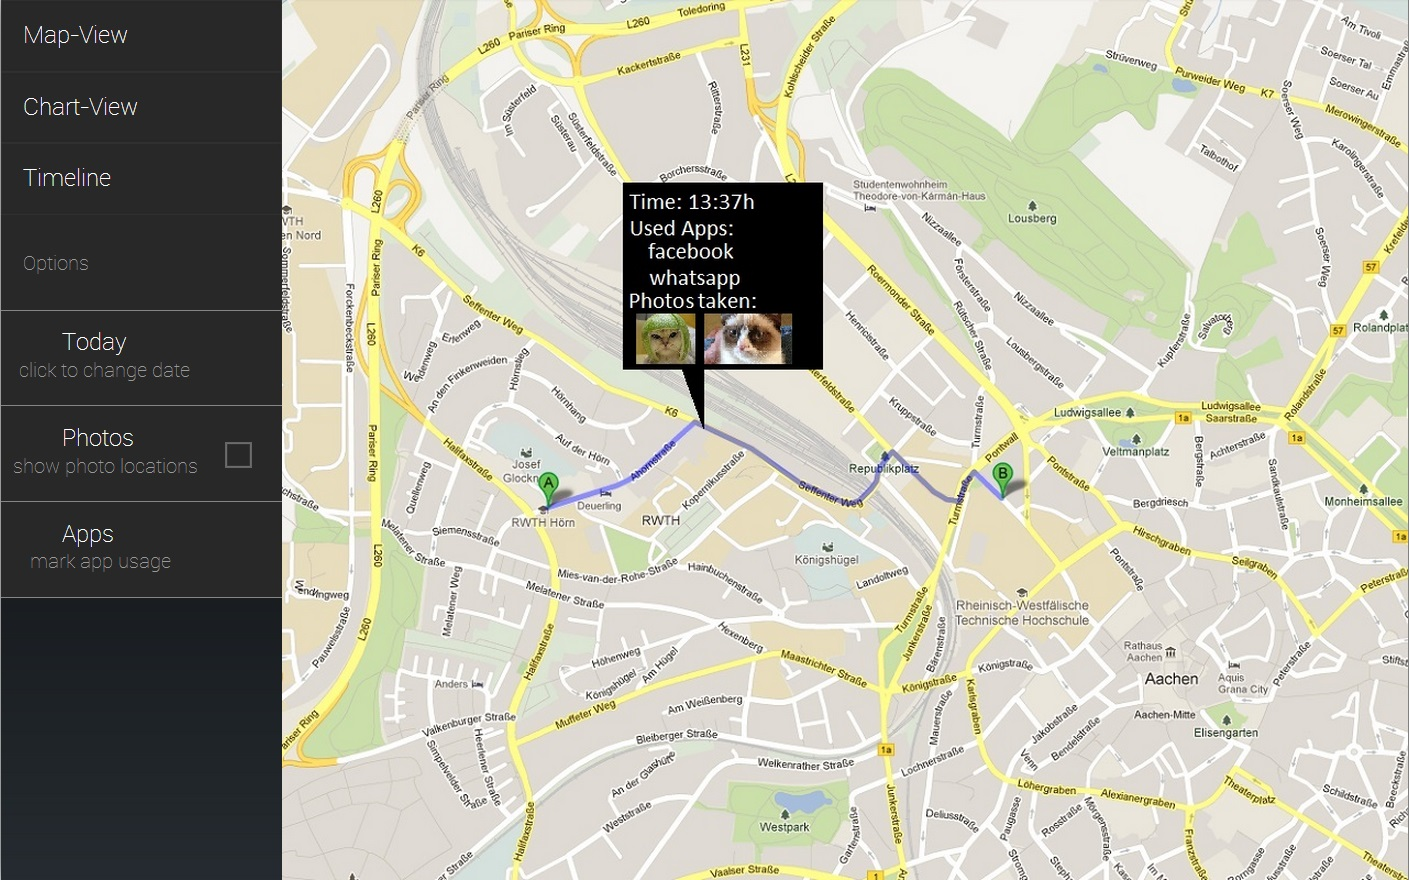
\includegraphics[width=\textwidth]{images/Design/1b_onClickPageView.jpg}
%\end{minipage}
\end{figure}

The second view, the chart view, shows the user his or hers daily activities in form of a pie chart.

\begin{figure}[h]
%\begin{minipage}[c][\textheight]{\textwidth}
	\caption{Chart-View}
	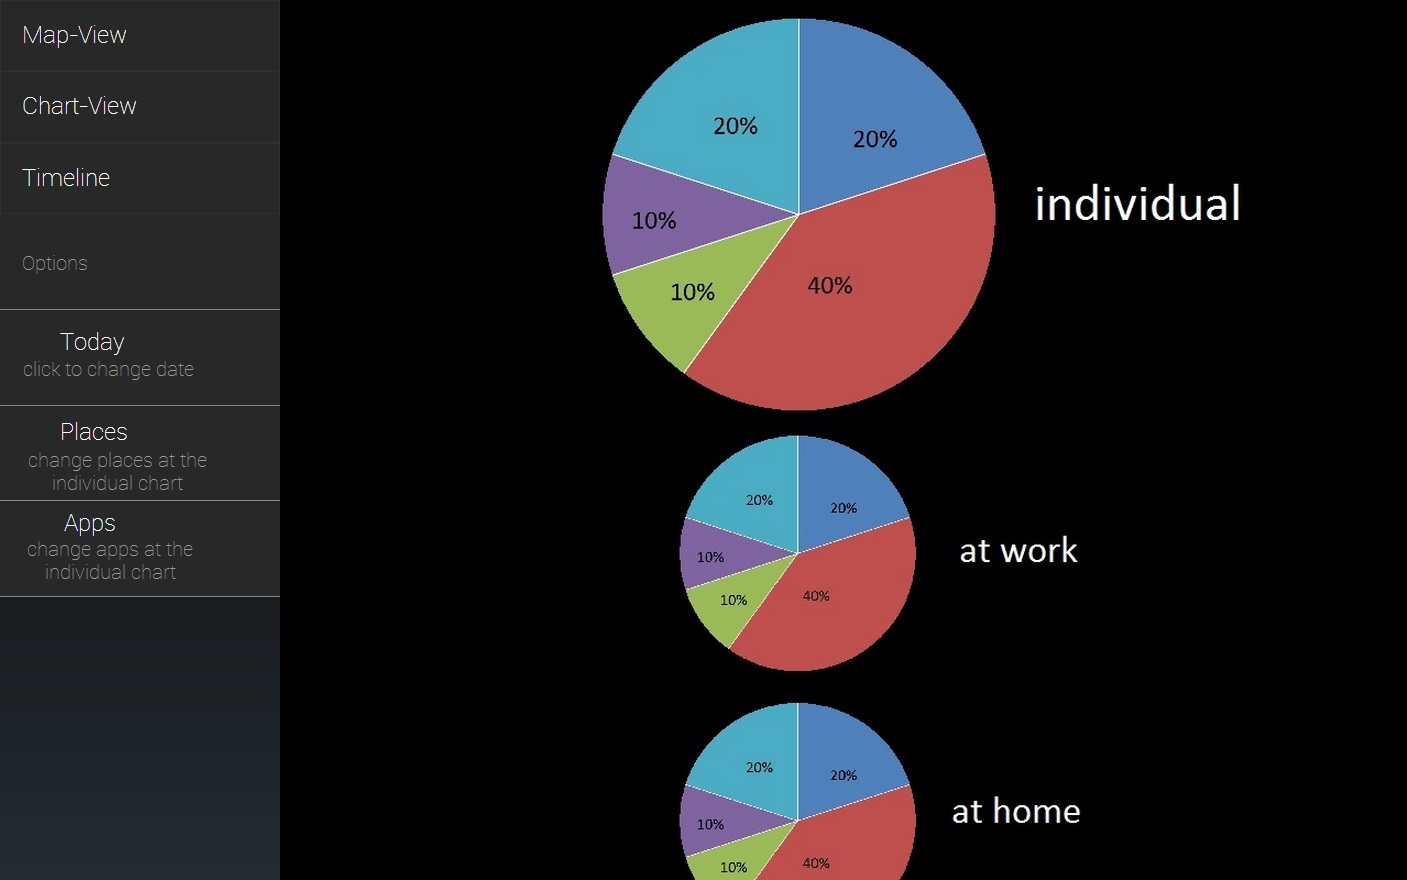
\includegraphics[width=\textwidth]{images/Design/2_ChartView.jpg}
%\end{minipage}
\end{figure}

\begin{figure}[h]
%\begin{minipage}[c][\textheight]{\textwidth}
	\caption{Timeline}
	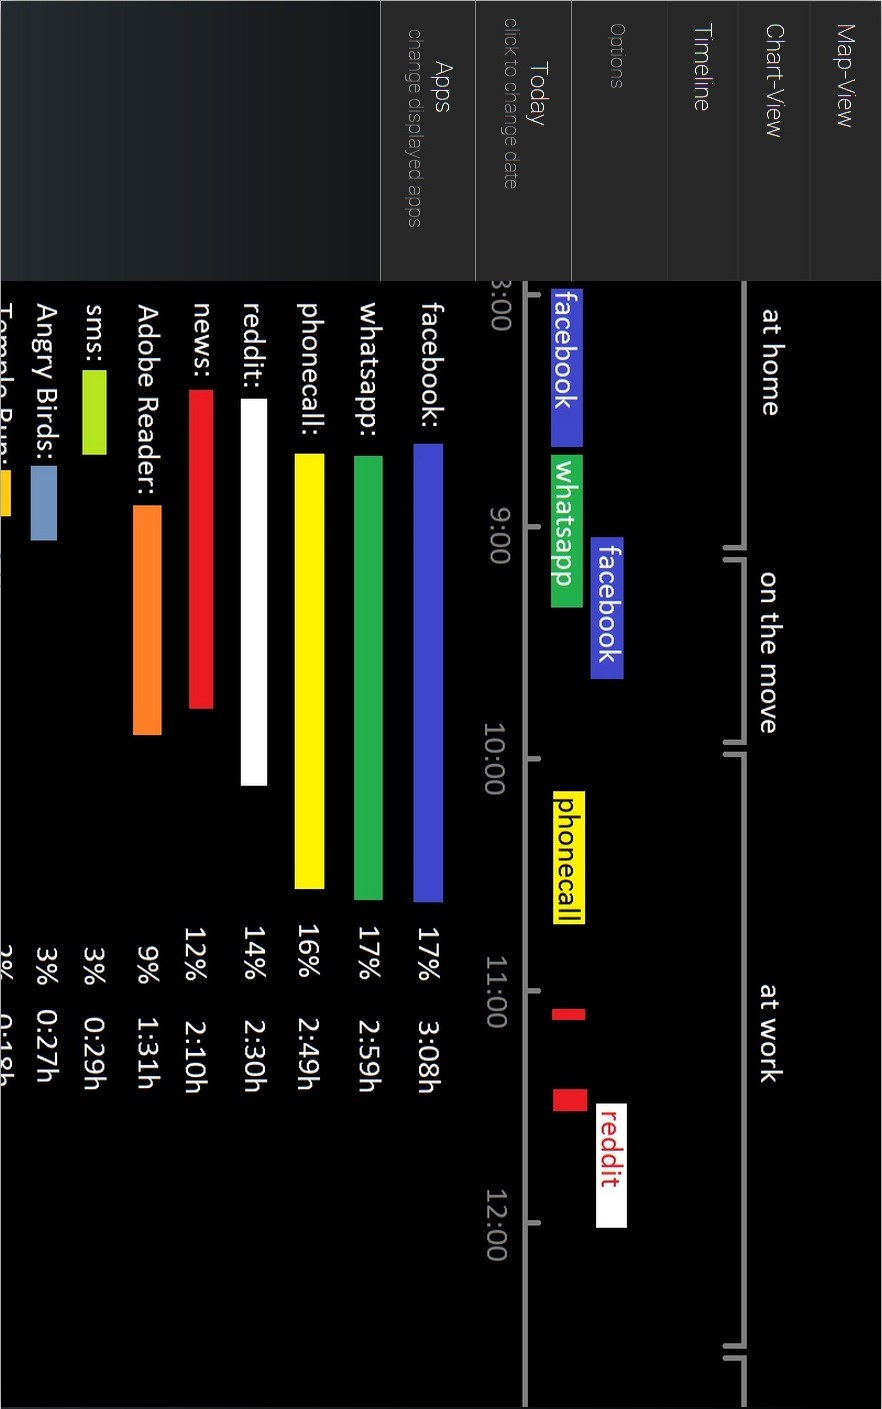
\includegraphics[width=\textwidth]{images/Design/3_TimeLine.jpg}
%\end{minipage}
\end{figure}

\newpage
\section{Time Schedule}
\label{subsec:time_schedule}

\newpage
\section{Basic Layout}

\newpage
\section{Data Management}

\newpage
\section{Mapview}

\newpage
\section{Chartview}

\newpage
\section{Timeline}
%
%The WaveLoc API, as described in chapter \ref{cha:waveloc_api}, offers functionalities to handle the information about the users that are stored in the database up to date, to provide data about participants of WaveLoc (users or POIs) that are close by, and it maintains the friends- and favorite-lists of every user.
%
%As \mnote{Transferring the API} already mentioned in section \ref{sec:waveloc_api__functionalities}, this API uses \emph{PHP}, \emph{MySQL} and runs on the web-server \emph{Apache}. It is possible to transfer this system from one server to another one by installing the whole set of files onto the destination server. One only has to adjust some rights, the content of some files, and to set up the database. The scripts have to get write access to the folders \texttt{/smarty/cache}, \texttt{/smarty/configs}, and \texttt{/smarty/templates\_c}. Thus, they have to get the required rights (\texttt{chmod 775}\footnote{Full rights for the root-user and the owner and rights to read/write for every other user}). The only three files that have to be adjusted are the \texttt{.htaccess} in the root directory of the API, the \texttt{/data/config.php}, and  \texttt{/data/server.php}. In the first file, only the domain has to be adjusted:
%
%\begin{lstlisting}
%ErrorDocument 404 http://wave.thues.com/404.htm
%\end{lstlisting}
%
%\pagebreak
%The second file contains six variables concerning the API that determine default values, among others:
%
%\begin{lstlisting}
%<?PHP
%	$mail_admin = "hendrik@thues.com";
%	// the title of the application
%	$appname = "WaveLoc";
%	// time when an inactive user is set offline
%	$idle_time_sec = "300";
%	// default radius
%	$std_radius = "300";
%	// default time to POI
%	$std_timetopoi = "15";
%	// distance of offline-users 
%	$max_distance = "31337000";
%?>
%\end{lstlisting}

\chapter{Evaluation}
\label{cha:evaluation}

To \mnote{Amount of test-persons} test and to improve the usability of WaveLoc, three sets of user-tests have been conducted. The first two with five users, the last one with three users. According to \citet{ruleof5}, it is sufficient to conduct user-tests with five users. Thus, 17 user-tests with different students (including the final set of tests (see chapter \ref{sec:evaluation__final_tests})) are more than required. As stated, the number of usability problems that are found in a test with $n$ users and a total number of $N$ problems is

$$N(1-(1-L)^n)$$

$L$ \mnote{Detecting most of the problems} denotes the proportion of usability problems discovered while testing a single user with a typical value of 31\%. According to this formula, about 84\% of the $N$ problems can be found if five users are tested. The second set of user-tests with five persons should reveal another 13\% of the original $N$ problems. Thus, conducting user-tests with 10 persons should result in finding about 97-98\% of the problems concerning the usability.

After conducting these three user-tests, a final test with 4 users has been conducted. The reason for this set was again to test the changes that have been implemented after each set of the first user-tests. The participants should consider the application operable intuitively.



The first two sets of user-tests have each been conducted with five students while the third one has been conducted with three students, each of them having different foreknowledge concerning smart phones.

\ldots{}
\part{}
\chapter{Related Work}
\label{cha:related_work}

This chapter will talk about another approach of visualizing the provided data. Thomas Honné's project of his Master thesis ``Interactive Visualizations of Activity Patterns in Learning Environments'' \cite{thomasthesis} will be discussed and compared to the result of this thesis, \emph{SmartDay}.

Honné's \mnote{Visualizing} project and thesis describe a way of visualizing daily activities with a special focus to learning environments. Both project try to visualize the data in different ways, \emph{SmartDay} in a native way on Android and Honnè's project in a non native way with the help of a website. Since both visualizations need access to the Internet, \emph{SmartDay} is able to store data locally and display them even without an Internet connection. But the website based service also has its pros, because most platforms provide a browser which is capable of displaying Java Script, which is mainly used for the website.

Because both projects use data provided by the same gathering application \emph{BigBrother}, this comparison can focus on only visualization as both projects have the same precondition.

Both \mnote{The map} projects use different views to represent the provided data and both use a map for position data. Honné's map shows, in contrast to the visualization of \emph{SmartDay}, visited locations as unconnected circles. These circles differ in size and get larger, the longer one uses applications at this point. Those circles can consist of more than one position data, meaning that one can adjust a size in meter in which all data will be merged into one circle. This forms clusters on the map and creates personal points of interest, showing the user in an intuitive way, where he or she has used his or hers device the most. The map in \emph{SmartDay} connects each point and does not weight them by total amount of times applications have been used. This can be helpful to reconstruct routes but can also look messy sometimes.\\
Thomas Honné's map view also provides further details when clicking on the circle. The user is then displayed with a small windows which shows a pie chart displaying the applications used grouped by their productivity level. Furthermore, a bar chart,  similar to the timeline's detail view, is displayed, ordered descending by total time of usage. And at last one can see all events that were tracked at this position, listed as text in chronological order. \emph{SmartDay} may have pie charts too, but these are in a separated view, not position based and are not directly accessed by the map view. The details and completeness of the website's view dominates the map view presented in the application.

The \mnote{Visualizing of patterns} website provides a section not included in the native application, called \emph{Patterns}. This section makes use of Iurii Ignatko's work to recognize patterns with the help data mining in the provided dataset \cite{iuriisthesis}. It displays connections between application usages, for example it may show you the pattern, that if you use the calendar application, you are likely to use email client afterwards. This can be helpful especially to track down the root of usage patterns which distract one from his or hers work.

Another \mnote{Productivity and line charts} of the website is a tab called \emph{Productivity}. This view displays the same data as the detail window of the map tab, but takes adjustable timespans as input. This is a good solution with respect to productivity, as one can directly see his or hers daily, weekly or monthly usage of productive and non productive applications. The view \emph{Line Chart} presents the user a view which displays a line chart representing the number of events over time. The chart is freely adjustable, as one can add lines with restrictions to events and applications, colorize them and select a timespan for the it. It is an interesting feature which allows to compare different activities and applications. 

The website's views are reasoned and well structured. Especially the map view has some clear advantages over the application's view. The general concept and use of position based charts is a step ahead of the applications visualization. But the website still has some unused potential. For example, the productivity tab should take time, date and position into account, when weighting an application's productivity, as it may be okay to play a game at 22:00 at home on a Friday evening. In addition, the website lacks of a view, where the user can see his or hers day in a chronological order, like it is done in the applications timeline.
\chapter{Conclusion}
\label{cha:conclusion}

%\chapterquote{Finally, in conclusion, let me say just this.}{Peter Sellers}
%
%This chapter summarises the whole process of developing the application WaveLoc. It depicts where problems occurred while implementing the application and which future work arises from this diploma thesis. 


\section{Review}

\newpage
%\label{sec:conclusion__review}
%
%The \mnote{WaveLoc's requirements} WaveLoc system enables its users to connect with each other and to find others that are nearby. These functionalities can be utilised to offer and to gain help among students. As backend that is used to handle the data and to exchange information such as images, documents, or videos, the service ... was proposed. This tool enables its users to communicate with each other, to share information, to discuss about specific topics, to create content collaboratively, and to store data location-based that may be accessed by others. \citet{ms2010} stated that ... is capable of being the basis of a PLE as depicted in the chapters \ref{sec:background__personal_learning_environment} and \ref{sec:background__google_wave_as_backend}.
%
%\ldots{}


% Set page to be wider for bibliography
\setwidesite{}

\begin{appendix} 

\addappheadtotoc

% Variant 1
\chapter{Bibliography}
\label{cha:bibliography}
\printbibliography[heading=offline,filter=offline]
\printbibliography[heading=online,filter=online]
% chapter bibliography (end)
% Variant 2
%\printbibliography


% \listoffigures

% \listoftables

%\lstlistoflistings

%\printglossary[title=Abbreviations]

%\chapter{Survey-Data}
\label{cha:survey_data}

\begin{enumerate2}
	\item \emph{Area of study} \newline
		\begin{table}[h!]
			\hspace{18pt}
			\begin{tabular}{l|rr}
				& Amount	& Percentage \\	
				\hline
				Computer Science				& 58		& 23.58\% \\
				Mechanical Engineering			& 15		& 6.10\% \\
				Waste Management Engineering	& 1			& 0.41\% \\
				Electronical Engineering		& 6			& 2.44\% \\
				Studying Languages				& 1			& 0.41\% \\
				Medical Engineering				& 3			& 1.22\% \\
				Studying to become a Teacher	& 20		& 8.13\% \\
				Mathematics						& 10		& 4.07\% \\
				Ergotherapy						& 1			& 0.41\% \\
				Business Administration			& 96		& 39.02\% \\
				Physics							& 2			& 0.81\% \\
				Biology							& 3			& 1.22\% \\
				Technical Communication			& 21		& 8.54\% \\
				Human Resources Management		& 1			& 0.41\% \\
				Chemistry						& 3			& 1.22\% \\
				Architecture					& 1			& 0.41\% \\
				Archaeology						& 1			& 0.41\% \\
				Geography						& 2			& 0.81\% \\
				Geology							& 1			& 0.41\% \\
				\hline
				Total:							& 246		& 100.00\% \\
			\end{tabular}
		\end{table}
	
		\clearpage
	
	\item \emph{Semester} \newline
		\begin{table}[h!]
			\hspace{18pt}
			\begin{tabular}{l|rr}
				& Amount	& Percentage \\	
				\hline
				1	& 3		& 1.20\% \\
				2	& 96	& 38.25\% \\
				3	& 10	& 3.98\% \\
				4	& 57	& 22.71\% \\
				5	& 5		& 1.99\% \\
				6	& 25	& 9.96\% \\
				7	& 7		& 2.79\% \\
				8	& 15	& 5.98\% \\
				9	& 5		& 1.99\% \\
				10	& 13	& 5.18\% \\
				11	& 0		& 0.00\% \\
				12	& 5		& 1.99\% \\
				13	& 2		& 0.80\% \\
				14	& 1		& 0.40\% \\
				15	& 1		& 0.40\% \\
				16	& 2		& 0.80\% \\
				17	& 0		& 0.00\% \\
				18	& 2		& 0.80\% \\
				19	& 1		& 0.40\% \\
				20	& 1		& 0.40\% \\
				\hline
				Total:							& 251		& 100.00\% \\
			\end{tabular}
		\end{table}



% \chapter{Listings}
\label{cha:listings}

\section{MySQL Database of the WaveLoc-API}
\label{sec:mysql_database_of_the_waveloc_api}
\lstinputlisting[label=code:serverdatabase,caption={},language=SQL]{listings/server_database.sql}\newpage




\end{appendix}

\backmatter

\end{document}
